\documentclass[11pt]{article}
\usepackage[margin=1in]{geometry}
\usepackage{amsmath,amssymb,booktabs,graphicx,microtype,url}
\usepackage[hidelinks]{hyperref}
\usepackage[numbers,sort&compress]{natbib}
\usepackage{caption}
\captionsetup{font=small}
\newcommand{\wc}{\mathrm{WC}}
\title{\textbf{Coverage Across the Horizon}\\[2pt]
\large Horizon- and Channel-Conditional Adaptive Conformal Calibration\\for Long-Term Time-Series Forecasting}
\author{Aarush Pandit\thanks{Vellore Institute of Technology, Vellore. Correspondence: \texttt{aarush093} on GitHub.} \and Nayan Jaggi \and Sree Dharinya S}
\date{}

\begin{document}
\maketitle

\begin{abstract}
Long-term time-series forecasting (LTSF) is evaluated almost entirely through deterministic point error. The three architectures that define the field---Informer, DLinear and PatchTST---disagree about nearly everything except this: none emits a predictive interval, at exactly the horizons where point forecasts are least trustworthy. Recent work has begun attaching conformal prediction to forecasters, but it is scored the way the point literature is scored: with one aggregate number. We show that this hides the failure that matters. We audit conditional coverage over a horizon-bucket $\times$ channel grid on the canonical LTSF suite and find that \emph{marginal coverage is uninformative}: the per-horizon split-conformal baseline (MSCP) attains the \emph{highest} marginal coverage of seven methods we compare (0.9123) and the \emph{worst} conditional coverage (worst-cell 0.7251), below a do-nothing global-conformal baseline at 0.7667. We then show that the obvious repair does not work either. Conditioning the conformal quantile on horizon and channel \emph{alone} makes worst-cell coverage worse (0.7588); adapting online \emph{alone} makes it worse still (0.7445). Only their combination helps, reaching 0.8657 with \emph{narrower} intervals and the best interval score of all seven methods---an interaction of $+0.1291$ that grows to $+0.3264$ on a harder 300-cell electricity-load surface where static conditioning collapses to 0.4621. The layer is post-hoc, distribution-free, model-agnostic and costs $0.22\,\mu$s per interval endpoint; no forecaster is trained. We report the price of whole-path coverage ($\approx$10$\times$ width), a decision-level evaluation in which interval gating wins only when misses cost $\gtrsim$5$\times$ false alarms, and a rolling-coverage analysis in which static conformal spends 17.5\% of a seasonal test period below 0.85 while the adaptive conditional layer never does. We also report, in full, an ablation-scoring artefact that initially reversed one of our conclusions.
\end{abstract}

\section{Introduction}

The modern LTSF literature is organised around a shared evaluation contract: deterministic point forecasts, scored by MSE and MAE, on a fixed benchmark suite, at horizons of 96 to 720 steps \citep{informer,dlinear,patchtst}. The three papers that define the field disagree about architecture almost completely---Informer argues for efficient attention, DLinear that a one-layer linear map beats it, PatchTST that attention wins again with patching and channel independence---and agree, silently, that no uncertainty need be reported. Because they disagree on everything else, the omission is a property of the field's evaluation contract rather than of any one paper. The ProbTS benchmark documents the resulting split directly: long-horizon point forecasting and short-horizon probabilistic estimation developed as separate literatures, with neither serving both needs \citep{probts}.

Conformal prediction is the natural repair. It is distribution-free, post-hoc, and requires no retraining, which matters when the forecaster is a frozen artefact---the normal deployment condition. A growing 2024--2026 line attaches conformal methods to forecasting: adaptive conformal inference for online coverage \citep{aci}, conformal PID control \citep{cpid}, autocorrelation-aware multi-step conformal prediction \citep{acmcp}, and joint multi-step constructions \citep{bellman,copulacpts}.

\paragraph{The problem this paper addresses.} That line has largely inherited the point literature's scoring habit. The closest benchmarking work to ours evaluates conformal methods for time series on marginal coverage, interval width and the Winkler score, and concludes that multi-step split conformal prediction is the best available method \citep{cpsurvey}. Its experiments use AutoARIMA on a monthly-sales corpus. We reproduce its ranking on our surface---and show that it inverts under conditional scoring. A method can hold 90\% coverage \emph{on average} while systematically failing at long horizons, on particular channels, or during particular seasons. Averages hide exactly the failures that make an interval worth having.

\paragraph{Contributions.}
\begin{enumerate}\itemsep2pt
\item \textbf{An audit.} A conditional-coverage map of the canonical LTSF suite over a horizon-bucket $\times$ channel grid, across seven interval methods and two frozen backbones (Section~\ref{sec:audit}). Marginal coverage and conditional coverage rank the methods in opposite orders.
\item \textbf{A method, and the finding that its two halves are inseparable.} A bucketed horizon $\times$ channel conditional adaptive conformal layer (Section~\ref{sec:method}). Conditioning alone and adaptation alone both \emph{underperform} the do-nothing baseline; their combination is worth $+0.1291$ worst-cell coverage on ETT and $+0.3264$ on electricity load (Section~\ref{sec:results}). We show the same interaction holds \emph{within} the conditioning, for the horizon axis specifically.
\item \textbf{The price of whole-path guarantees.} Every per-step method gives essentially zero probability that an entire 720-step trajectory is covered. Restoring $\approx$0.91 whole-path coverage costs $\approx$10$\times$ the interval width (Section~\ref{sec:joint}).
\item \textbf{A decision-level evaluation, reported in both directions.} On interval-gated peak-load flagging, calibrated intervals beat a point-forecast rule only when misses cost at least $\approx$5$\times$ false alarms; below that the point rule is cheaper, and a worst-channel interval rule is worse than doing nothing (Section~\ref{sec:decision}).
\item \textbf{A negative methodological result we think is reusable.} Scoring a bucket-count ablation on each setting's own grid reverses its conclusion, because worst-cell coverage is a minimum over cells and coarser grids have fewer cells (Section~\ref{sec:frailty}). We found this after the confounded figure had been presented, and report it in full.
\end{enumerate}

\section{Related work and positioning}

\paragraph{Conformal prediction for time series.} Split conformal prediction assumes exchangeability, which time series violate. Adaptive conformal inference (ACI) responds by updating the target level online from realised coverage, guaranteeing long-run coverage without distributional assumptions \citep{aci}; conformal PID control generalises the update \citep{cpid}. Multi-step variants calibrate per horizon (MSCP) or model cross-horizon error dependence \citep{acmcp,o2cp}. Joint constructions target whole-trajectory coverage through dynamic programming \citep{bellman} or copulas \citep{copulacpts}. Conditional guarantees have been formalised in the regression setting \citep{gcc}, and exact distribution-free conditional coverage is known to be impossible in general \citep{gcc}.

\paragraph{What is new here.} We are not the first to condition conformal intervals per horizon; MSCP is an established baseline and we treat it as one throughout. We are not the first to adapt online; ACI is prior work and one of our ablation arms. The contribution is (i) that these are evaluated on the LTSF grid at scale under conditional scoring, where their individual behaviour turns out to be \emph{negative}; and (ii) that their combination is what works, which no prior work reports because no prior work runs the $2\times2$.

\paragraph{Nearest neighbours.} \citet{cpsurvey} is the closest benchmarking work and provides our central foil (Section~\ref{sec:audit}); it uses AutoARIMA on monthly sales and marginal metrics only, so it overlaps our setting in neither data, backbone, nor metric. BC-ACI \citep{bcaci} is the closest method on the adaptation axis: it estimates forecast bias online per horizon and re-centres the interval. It moves the interval's \emph{centre}; we condition its \emph{width}, and it has no channel dimension. We measure its premise directly on our surface in Section~\ref{sec:bias}. DeRegiME \citep{deregime} is the nearest work by data and backbone---probabilistic forecasting on the same suite with DLinear and PatchTST encoders---but it trains a parametric density model optimising NLPD and CRPS, whereas we perform distribution-free post-hoc calibration with coverage control and train nothing. Concurrent work on gate-localised conformal prediction \citep{glcp} couples calibration to a learned representation and likewise trains its own forecasting module.

\section{Setup}\label{sec:setup}

\paragraph{Backbones.} We use DLinear \citep{dlinear} and NLinear as frozen point forecasters, fitted once per (dataset, horizon) by closed-form regularised least squares and never updated. \textbf{This is a deviation from our pre-registered plan}, which specified DLinear, PatchTST and Informer; the two Transformer backbones were dropped under a compute-contraction rule and NLinear substituted. The substitution is recorded as a deviation rather than a design choice, and Section~\ref{sec:limitations} states what it costs the model-agnosticism claim. Because the fit is closed-form, it is deterministic: the usual multi-seed requirement is vacuous for the fitting step, and we publish the single seed (2026) used for all stochastic components.

\paragraph{Data and protocol.} ETTh1, ETTh2, ETTm1, ETTm2 at $H \in \{96,192,336,720\}$ form the main study (32 configurations). A case study uses the LTSF Electricity benchmark, screened to 50 of 321 meters (Section~\ref{sec:casestudy}). Splits are strictly sequential in time, never random; \texttt{drop\_last} batch truncation is disabled everywhere, since it is known to inflate reported LTSF scores; calibration windows are strided rather than overlapping, to limit residual dependence between adjacent windows. We verified the split ordering and the absence of look-ahead directly: perturbing the second half of the test block leaves every method's first-half intervals bit-identical.

\paragraph{Point-forecast sanity.} DLinear reaches MSE 0.3702 / 0.4041 / 0.4334 / 0.4714 on ETTh1 at $H=96/192/336/720$, within about 1.3\% of published values. One configuration disagrees: ETTh2 at $H=720$ measures 0.7407 against published figures that disagree among themselves (roughly 0.605 to 0.831), plausibly a look-back-length difference. We flag it rather than select the comparison that flatters us.

\paragraph{Metrics.} Let $\alpha=0.10$. For a residual tensor $R \in \mathbb{R}^{n \times H \times C}$ and half-widths $\hat q$, empirical coverage on cell $(k,c)$ is the fraction of test paths and steps in horizon bucket $k$, channel $c$, with $|R| \le \hat q$. We report \emph{marginal} coverage; \emph{worst-cell} coverage $\wc = \min_{k,c}$; and, because a minimum over a wide grid is a noisy statistic, the 5th percentile of the cell distribution, the fraction of cells within $\pm5$ points of target, and the fraction below 0.80. We also report normalised width, the Winkler interval score, whole-path (joint) coverage, and calibration-layer wall-clock cost.

\paragraph{Reproducibility.} A clean clone of the released repository, re-run end to end, reproduces the committed result file across all 12{,}625 numeric values with maximum absolute deviation $0.0$ on the reference machine; across machines the numbers agree to four decimal places, with residual deviations at the $10^{-13}$ level attributable to floating-point summation order. Every number in this paper is generated from the released artefacts by a script, not transcribed.

\section{Method}\label{sec:method}

The layer sits entirely downstream of a frozen forecaster and is implementable in NumPy.

\paragraph{Nonconformity.} Residuals are normalised by a rolling per-channel scale $s_c$ (median absolute deviation, floored at $10^{-8}$), giving scores $S = |R| / s_c$. The MAD-versus-standard-deviation choice is an ablation (Section~\ref{sec:ablations}).

\paragraph{Bucketed conditioning.} Fitting $H$ independent quantiles for $H=720$ on a calibration block of order $10^2$ paths explodes variance. We therefore partition the horizon into $K$ log-spaced buckets, so that early steps---where residual scale changes fastest---get fine resolution and late steps are pooled. For $H=720, K=6$ the edges are $[1,3,9,27,80,240,720]$. Conditioning is on the product grid (bucket $\times$ channel): $K \times C$ cells, $42$ on ETT and $300$ on the electricity surface. $K$ is an ablation (Section~\ref{sec:frailty}).

\paragraph{Split-conformal quantile.} Within each cell we use the exact finite-sample conformal quantile: with $n$ calibration scores, take the $\lceil (n+1)(1-\alpha) \rceil / n$ empirical quantile, upper-interpolated.

\paragraph{Online adaptation.} Each cell carries its own ACI-style tracker. After observing whether the interval covered, the cell's working level is updated by $\alpha_{t+1} = \alpha_t + \gamma\,(\alpha - \mathbf{1}\{\text{miss}\})$ with $\gamma$ a step size and $\alpha_t$ clamped to $[10^{-4}, 0.5]$, and the interval is re-read from that cell's own empirical score distribution. The tracker is per-cell: this is the only structural difference from ACI, and Section~\ref{sec:results} shows it is the difference that matters.

\paragraph{Cost.} The full layer---all seven methods, ETTh1 at $H=720$---runs in 102\,ms, or $0.22\,\mu$s per interval endpoint. The calibration layer is negligible beside the forecaster.

\paragraph{Theory scope.} We claim only what this construction supports: ACI-family \emph{long-run} adaptive coverage, plus \emph{approximate} conditioning at bucket resolution. We do not claim finite-sample validity under distribution shift, and we do not claim exact conditional coverage, which is impossible distribution-free in general \citep{gcc}. Bucketing is a variance-control device, not a guarantee.

\section{The audit: marginal coverage is uninformative}\label{sec:audit}

Table~\ref{tab:main} compares seven interval methods spanning the $2\times2$ of conditioning and adaptation, plus a Gaussian-residual and an MSCP baseline.

\begin{table}[t]\centering\small
\caption{Main study: ETT $\times$ 4, 42-cell grid, target 0.90, mean over 32 configurations. Every method is marginally calibrated; they differ by 14 points of worst-cell coverage. Joint = whole-path coverage.}
\label{tab:main}
\begin{tabular}{llccccc}
\toprule
Method & Conditioning / adaptive & Marginal & Worst-cell & Width & Winkler & Joint\\
\midrule
Gaussian residual & $H\times C$ / no & 0.9096 & 0.7762 & 2.0254 & 2.6804 & 0.0045\\
Global split CP & none / no & 0.9097 & 0.7667 & 2.0857 & 2.9422 & 0.0034\\
Per-horizon (MSCP) & horizon / no & \textbf{0.9123} & \textbf{0.7251} & 2.0392 & 2.7649 & 0.0018\\
Channel-only & channel / no & 0.9099 & 0.7797 & 2.1711 & 2.9806 & 0.0034\\
Static conditional & $H\times C$ / no & 0.9084 & 0.7588 & 2.1304 & 2.9095 & 0.0010\\
ACI & none / yes & 0.9031 & 0.7445 & 1.8742 & 2.8310 & 0.0016\\
\textbf{Proposed} & $H\times C$ / yes & 0.9098 & \textbf{0.8657} & 1.9245 & \textbf{2.6366} & 0.0005\\
\bottomrule
\end{tabular}
\end{table}

Read the marginal column alone and the seven methods are indistinguishable: every one lands within 0.9 points of the 90\% target. Read the worst-cell column and they span fourteen points.

\paragraph{The ranking inverts.} MSCP has the \emph{best} marginal coverage in the table and the \emph{worst} conditional coverage---0.7251, fully four points below simply using one global quantile. This is not a quirk of our implementation: it is what \citet{cpsurvey} would conclude from our data, since that benchmark scores marginal coverage, width and Winkler, on all three of which MSCP is competitive here. Per-horizon conditioning spends a fixed calibration budget across $H$ separate quantiles, so each is estimated from fewer effective samples; the resulting variance shows up precisely in the minimum. A benchmark that reports only aggregate statistics cannot see this, and will recommend the method that fails hardest per cell.

\section{Results: the interaction is the finding}\label{sec:results}

The four rows of the $2\times2$ in Table~\ref{tab:main} are the experiment:
\[
\underbrace{0.7667}_{\text{neither}} \quad
\underbrace{0.7588}_{\text{conditioning only}} \quad
\underbrace{0.7445}_{\text{adaptation only}} \quad
\underbrace{0.8657}_{\text{both}}
\]
Each single intervention makes worst-cell coverage \emph{worse} than the do-nothing baseline. The interaction term is
\[
\text{P} - \text{C} - \text{A} + \text{G} = 0.8657 - 0.7588 - 0.7445 + 0.7667 = +0.1291 .
\]

The mechanism is intelligible. Conditioning alone slices a finite calibration block into 42 cells, and each cell's static quantile is estimated from too little data---variance, concentrated in the minimum. Adaptation alone has enough data but only one global knob, so it cannot move a cell that is failing while the aggregate looks healthy; it purchases marginal coverage by narrowing (width 1.8742, the narrowest in the table) and its worst cell degrades. Together, conditioning supplies the resolution to see per-cell failure and adaptation supplies the correction, so the variance that sinks static conditioning is continuously repaired.

This is not bought with width. Proposed is \emph{narrower} than the global baseline (1.9245 vs.\ 2.0857) and attains the best Winkler score of all seven methods (2.6366), which jointly penalises width and misses.

\paragraph{Consistency.} Against MSCP, static conditional and ACI, Proposed wins on worst-cell in 32 of 32 configurations; against global conformal and channel-only, 31 of 32; against the Gaussian baseline, 26 of 32. The gain is present at every horizon and does not come only from long ones ($+0.1043$, $+0.1238$, $+0.0932$, $+0.0747$ at $H = 96, 192, 336, 720$).

\paragraph{Backbone independence.} The layer never sees the forecaster. Swapping DLinear for NLinear, Proposed reaches worst-cell 0.8664 and 0.8651 respectively---within 0.0013---while the global baseline moves by 3.2 points (0.7510 vs.\ 0.7825). The two backbones have materially different error processes (Section~\ref{sec:bias}), which makes the agreement stronger evidence than two backbones that merely share a name.

\section{Both halves of the conditioning need the adaptation}\label{sec:frailty}

Setting $K=1$ collapses the horizon axis, leaving channel-only conditioning; we verified structurally that Proposed at $K=1$ equals the channel-only adaptive arm exactly in all 32 configurations. Sweeping $K$ on a \emph{fixed} scoring grid:

\begin{center}\small
\begin{tabular}{lcc c}
\toprule
& $K=1$ (channel only) & $K=6$ (horizon $\times$ channel) & effect of the horizon axis\\
\midrule
Static (Cond) & 0.7797 & 0.7588 & $-0.0209$\\
Adaptive (Proposed) & 0.8263 & 0.8657 & $+0.0394$\\
\bottomrule
\end{tabular}
\end{center}

The horizon axis \emph{hurts} without adaptation and \emph{helps} with it: a second interaction of $+0.0603$, with $K=6$ beating $K=1$ in 31 of 32 configurations on the adaptive arm. The same structure appears on the electricity surface, more strongly: $-0.0853$ static, $-0.0034$ adaptive, interaction $+0.0818$.

\paragraph{A scoring artefact that reversed this conclusion.} Our first $K$ ablation scored each $K$ on \emph{its own} grid. Worst-cell coverage is a minimum over $K \times C$ cells---7 cells at $K=1$, 70 at $K=10$---and a minimum over fewer, larger cells is higher almost by construction. Own-grid scoring therefore decreases monotonically in $K$ (0.8717 at $K{=}1$ to 0.8616 at $K{=}10$) and recommends discarding the horizon axis; fixed-grid scoring recommends $K=6$. The sign test flips completely: $K=6$ beats $K=1$ in 31/32 configurations on a fixed grid and 0/32 on own grids. The two agree exactly at $K=6$, where the grids coincide, which is the consistency check that nothing else moved.

We report this because the confounded figure was presented before the error was found, and because the general rule is reusable: \textbf{never compare a minimum or maximum across settings that change the number of cells it is taken over.} The same principle governs our cross-surface comparisons, where a minimum over 300 cells is not comparable to a minimum over 42.

\section{Case study: electricity load under seasonal shift}\label{sec:casestudy}

We screen the 321-client LTSF Electricity benchmark to meters with no zero readings---a measured criterion, not an assumed one: 92 of 321 qualify and we keep the first 50, yielding a 300-cell grid. Calibration falls in late winter and spring; the test block runs from late spring through the end of the year, so the evaluation crosses a genuine seasonal transition rather than a synthetic one.

\begin{table}[t]\centering\small
\caption{Electricity, 50 meters, 300-cell grid, mean over 8 configurations. Distributional grid statistics are reported alongside the minimum because a minimum over 300 cells is a noisy statistic.}
\label{tab:ecl}
\begin{tabular}{lccccc}
\toprule
Method & Marginal & Worst-cell & 5th pct.\ cell & Within $\pm$5 pt & Winkler\\
\midrule
Gaussian residual & 0.8330 & 0.4270 & 0.6314 & 0.500 & 1.6702\\
Global split CP & 0.8644 & 0.5757 & 0.7995 & 0.534 & 1.5264\\
Per-horizon (MSCP) & 0.8472 & 0.5382 & 0.7158 & 0.511 & 1.5925\\
Channel-only & 0.8629 & 0.5473 & 0.7860 & 0.525 & 1.5456\\
Static conditional & 0.8610 & 0.4621 & 0.6725 & 0.522 & 1.5417\\
ACI & 0.8921 & 0.6177 & 0.8353 & 0.488 & 1.5152\\
\textbf{Proposed} & 0.8964 & \textbf{0.8306} & \textbf{0.8806} & \textbf{0.977} & \textbf{1.4083}\\
\bottomrule
\end{tabular}
\end{table}

The pattern of Section~\ref{sec:results} sharpens. Static conditioning is now actively harmful (0.4621, thirteen points below the global baseline); adaptation alone recovers part of it (0.6177); the combination reaches 0.8306. The interaction is $+0.3264$, two and a half times its ETT value. The distributional statistics move together with the minimum: 97.7\% of the 300 cells land within five points of target under Proposed, against 53.4\% under global conformal.

\subsection{Adaptation, observed rather than averaged}\label{sec:traces}

A block average cannot distinguish a method that holds target from one that over-covers and then collapses. Figure~\ref{fig:traces} plots rolling coverage through the test block.

\begin{figure}[t]\centering
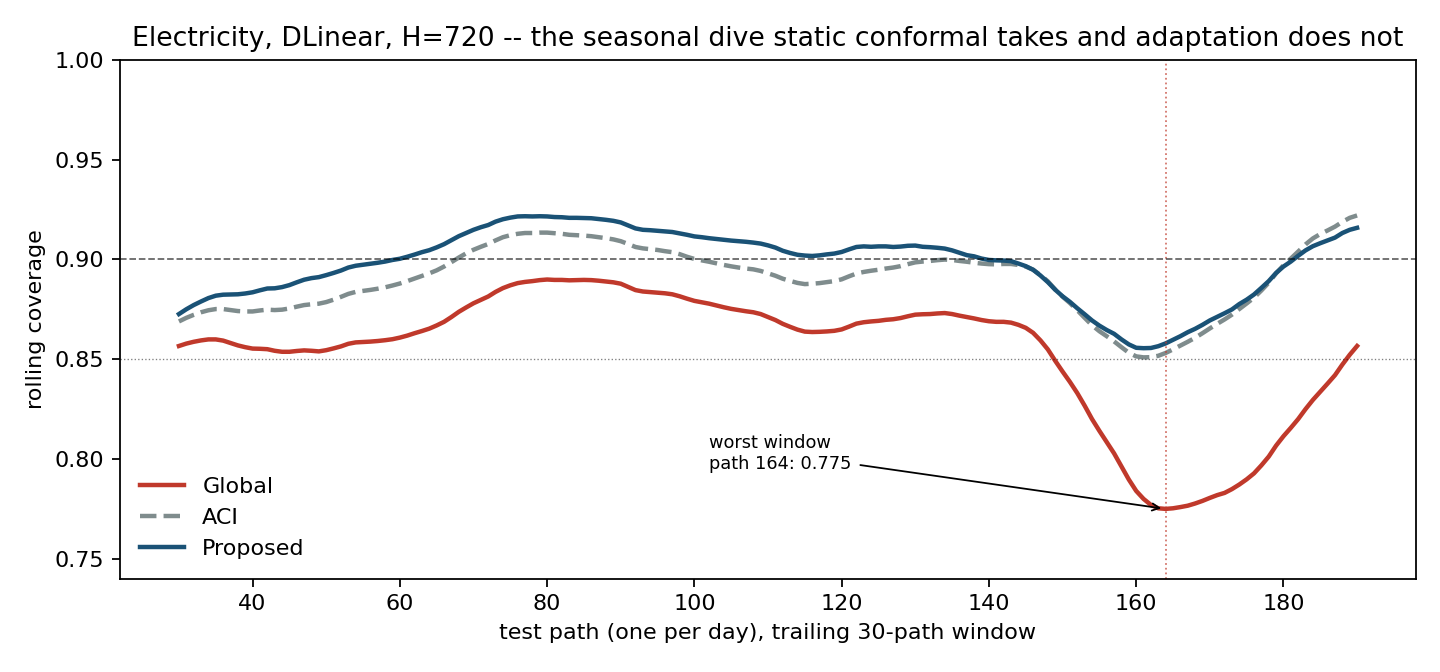
\includegraphics[width=0.86\textwidth]{fig_traces.png}
\caption{Rolling 30-day coverage, Electricity, DLinear, $H=720$. Static global conformal dives through the autumn transition, bottoming at 0.7750; the conditional adaptive layer holds 0.8579 through the identical window on identical forecasts.}
\label{fig:traces}
\end{figure}

Across the eight electricity configurations, global conformal spends 17.5\% of the test period below 0.85 coverage, with excursions averaging 21.8 days; ACI and Proposed spend 0.0\% there, with longest excursion zero. The static failure is not diffuse: its worst window falls at test path 163--164 in seven of eight configurations, at the same point for both backbones, i.e.\ it is a property of the data. It deepens with horizon, to 0.7750 at $H=720$.

\paragraph{Reported against ourselves.} On ETT, whose split does not cross a season, the effect is much weaker---global 16.0\% below 0.85, Proposed 11.9\%---and \emph{ACI alone is worse than doing nothing} (17.1\%). Adaptation is not a free win; it is the interaction again, from a third direction.

\subsection{How much calibration data does this need?}\label{sec:calwindow}

Truncating the calibration block from the front (keeping the most recent paths) separates a structural limitation from a statistical one. On ETT, Proposed leads every baseline at every size, including at $n_{\text{cal}}=28$ (0.7461 against the best baseline's 0.6685). On electricity the two failure modes separate cleanly: across a fourfold increase in calibration data the global baseline gains 0.034 of worst-cell and MSCP 0.008, while Proposed gains 0.200 (0.6307 $\rightarrow$ 0.8306) and has \emph{not} saturated (Figure~\ref{fig:calwindow}). The baselines' failure is structural---they have no mechanism that more data would help; ours is statistical---it is estimating a 300-cell grid from fewer than a hundred paths. Our reported 0.8306 is therefore a floor, not a ceiling, and the honest limitation is that wide grids need data.

\begin{figure}[t]\centering
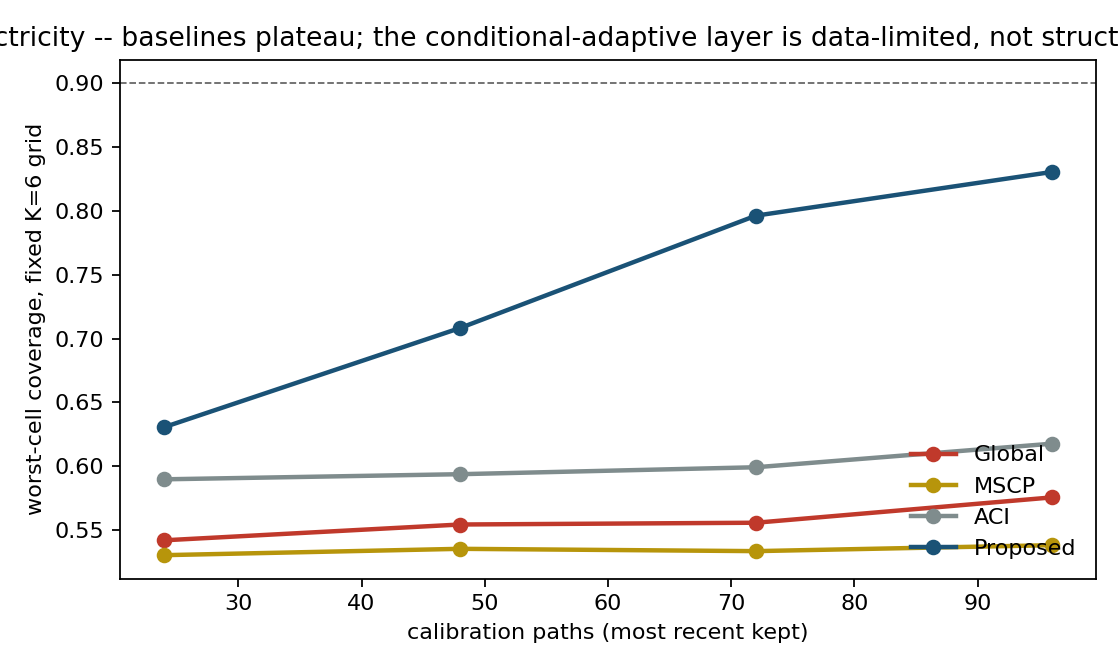
\includegraphics[width=0.72\textwidth]{fig_calwindow.png}
\caption{Worst-cell coverage against calibration size, Electricity. Baselines plateau; the conditional adaptive layer is data-limited, not structure-limited.}
\label{fig:calwindow}
\end{figure}

\section{Whole-path coverage and its price}\label{sec:joint}

Per-cell 90\% coverage is not 90\% coverage of an entire trajectory, and conflating the two would be a serious overclaim. We measure both. Every per-step method in Table~\ref{tab:main} achieves essentially zero joint coverage: the probability that all 720 steps across all channels are simultaneously covered is 0.0005 for Proposed and at most 0.0045 for any method. Applying a max-normalised-score layer restores whole-path coverage to 0.9124 at $10.16\times$ the width; a Bonferroni layer gives 0.9130 at $10.19\times$. Whole-path coverage on the LTSF grid is available, and it costs an order of magnitude in width. That is a finding about the regime, not a defect of any method---and it is why we report both numbers rather than the flattering one.

Joint coverage is also strongly finite-sample. Holding calibration size fixed at 80 paths, whole-path coverage is 0.9259 at $H=96$ against 0.8947 at $H=720$, so the observed decay across horizons is roughly 62\% horizon effect and 38\% sample-size effect. At $H=720$, halving calibration from 80 to 40 paths drops joint coverage from 0.8947 to 0.5632.

\section{Decision-level evaluation}\label{sec:decision}

Coverage is instrumental. We evaluate interval-gated peak-load flagging: a peak threshold is set on the calibration block only (we verified by source inspection and by perturbation that no test data enters it), and a meter-hour is flagged when the forecast, or the upper interval endpoint, exceeds it. Costs are normalised so that flagging nothing costs 1.0.

\begin{center}\small
\begin{tabular}{lccc}
\toprule
Miss\,:\,false-alarm & Point forecast & Interval (global) & Interval (Proposed)\\
\midrule
2:1 & \textbf{0.4625} & 0.6703 & 0.6919\\
5:1 & 0.3872 & 0.2988 & \textbf{0.2981}\\
10:1 & 0.3621 & 0.1749 & \textbf{0.1668}\\
20:1 & 0.3495 & 0.1130 & \textbf{0.1012}\\
50:1 & 0.3420 & 0.0758 & \textbf{0.0618}\\
\bottomrule
\end{tabular}
\end{center}

Calibrated intervals are not universally better. At 2:1 the point rule is cheaper, because interval gating flags aggressively and pays for it in false alarms. From roughly 5:1 the ordering reverses and widens: at 10:1 the proposed layer costs 0.1668 against the point rule's 0.3621, catching materially more peaks at lower total cost. We also report the worst-channel cost, where the picture is worse: at 2:1 the interval rules reach 8--10$\times$ the do-nothing cost on their worst channel. Interval gating is a tool for asymmetric-cost regimes, and we report the regime where it loses as plainly as the one where it wins.

\section{Ablations and diagnostics}\label{sec:ablations}

\paragraph{Adaptation step size.} Worst-cell coverage rises monotonically with $\gamma$ (0.652 at $\gamma=0$, 0.7546 at 0.005, 0.8571 at 0.02, 0.8791 at 0.05, 0.8901 at 0.1) while width falls (3.5677 to 2.3627). We use $\gamma=0.05$ throughout; the trend indicates the result is not a knife-edge tuning artefact.

\paragraph{Scale estimator.} With MAD normalisation the global baseline reaches 0.8549 worst-cell against 0.6869 with standard deviation, while Proposed is invariant at 0.8571---the conditional adaptive layer absorbs a choice that materially changes the baseline.

\paragraph{Stride.} Our default calibration stride of 24 steps is a deviation from the strictest non-overlap reading of our protocol, taken because strict non-overlap at $H=96$ leaves only 30 calibration paths. Across strides 24 / 48 / 96 ($n_{\text{cal}} = 117 / 59 / 30$), Proposed scores 0.8702 / 0.8382 / 0.7500 and leads at every stride. The ordering is stable; the level falls with sample size, consistent with Section~\ref{sec:calwindow}.

\subsection{Is the gain just absorbing forecast bias?}\label{sec:bias}

BC-ACI \citep{bcaci} argues that a frozen forecaster develops persistent bias after a shift, and that symmetric intervals then pay a width overhead of roughly twice the bias. Our intervals are symmetric and our case-study split is seasonal, so the premise applies and we tested it.

The answer splits by backbone. DLinear carries per-cell bias of 16.5\% of interval width on ETT, and it \emph{persists}: calibration-block bias predicts test-block bias at $r=+0.579$ (ETT) and $+0.731$ (electricity), growing with horizon. NLinear carries 4.2\% and no persistence ($r=-0.044$, $-0.595$). The mechanism is architectural: NLinear subtracts the last observed value and re-anchors each window, while DLinear decomposes trend and seasonality and drifts.

Two conclusions follow. First, a leakage-free re-centring buys \emph{width}, not \emph{coverage}: on the worst DLinear configuration it returns 11.2\% of width while moving worst-cell coverage the wrong way (0.8547 $\rightarrow$ 0.8451). Bias correction is orthogonal to our objective and composable with our layer, since it acts on the score and we act on the quantile. Second, and more usefully, this rules out an alternative explanation for Section~\ref{sec:frailty}: if the horizon axis were merely soaking up horizon-dependent bias, its benefit would be far larger on DLinear, which carries $3.5\times$ the bias. It is not---$+0.0406$ on DLinear against $+0.0383$ on NLinear---and per configuration the association is slightly \emph{negative} ($r=-0.317$). The horizon axis is capturing scale heterogeneity, consistent with the observation that per-horizon interval width is strongly daily-periodic (lag-24 autocorrelation $+0.9810$) rather than monotone in $h$.

\section{Limitations}\label{sec:limitations}

\textbf{Backbones.} We evaluate two linear forecasters, not the Transformer architectures our study was designed around. The model-agnosticism claim is therefore supported across two backbones with genuinely different error processes, but not across architectural families. The decisive test is PatchTST, which enforces channel independence by construction: if the channel axis is where calibration breaks, a channel-independent backbone should either shrink the gain (it already separates channels) or enlarge it (it never pools statistical strength). Either result is informative and neither is available here.

\textbf{Guarantees.} We claim long-run adaptive coverage and approximate bucketed conditioning, nothing stronger. Exact conditional coverage is unattainable distribution-free \citep{gcc}, and our finite-sample marginal guarantee does not survive the non-exchangeability we deliberately evaluate under.

\textbf{Grid width.} Worst-cell coverage over 300 cells is not comparable to worst-cell coverage over 42; we report distributional statistics alongside, and we do not compare minima across surfaces.

\textbf{Sample size.} On the 300-cell surface the method has not saturated in calibration data. Reported electricity numbers are lower bounds on what the layer achieves with a longer calibration block.

\textbf{One reproduction discrepancy.} ETTh2 at $H=720$ (Section~\ref{sec:setup}) remains unresolved against inconsistent published baselines.

\section{Conclusion}

Attaching conformal prediction to an LTSF forecaster is easy; attaching it so that coverage holds \emph{where it is needed} is not. Scored marginally, seven interval methods are indistinguishable and the ranking recommends the one that fails hardest per cell. Scored conditionally, the obvious individual repairs---condition the quantile, or adapt it online---each make things worse than doing nothing. What works is the combination, by a margin that grows as the grid gets harder, at negligible computational cost and without touching the forecaster.

We think the transferable lesson is about evaluation rather than about our particular layer. A single aggregate coverage number is compatible with systematic failure along horizon, channel and season; and a minimum computed over a grid is not comparable across settings that change the grid. Both of these bit us before they became findings, and both are cheap to check.

\paragraph{Reproducibility.} Code, all result artefacts, the generated results summary, and the complete decision, failure and open-question registers---including the two lost-work incidents and the scoring confound described above---are released at \url{https://github.com/aarush093/coverage-across-the-horizon}. The main study runs in under four minutes on CPU.

\small
\begin{thebibliography}{99}
\bibitem[Zhou et al.(2021)]{informer} H.~Zhou et al. Informer: Beyond efficient Transformer for long sequence time-series forecasting. \emph{AAAI}, 2021.
\bibitem[Zeng et al.(2023)]{dlinear} A.~Zeng, M.~Chen, L.~Zhang, Q.~Xu. Are Transformers effective for time series forecasting? \emph{AAAI}, 2023.
\bibitem[Nie et al.(2023)]{patchtst} Y.~Nie, N.~H.~Nguyen, P.~Sinthong, J.~Kalagnanam. A time series is worth 64 words. \emph{ICLR}, 2023.
\bibitem[Zhang et al.(2024)]{probts} J.~Zhang et al. ProbTS: Benchmarking point and distributional forecasting. \emph{NeurIPS Datasets \& Benchmarks}, 2024.
\bibitem[Gibbs \& Cand\`es(2021)]{aci} I.~Gibbs, E.~Cand\`es. Adaptive conformal inference under distribution shift. \emph{NeurIPS}, 2021.
\bibitem[Angelopoulos et al.(2023)]{cpid} A.~Angelopoulos, E.~Cand\`es, R.~Tibshirani. Conformal PID control for time series prediction. \emph{NeurIPS}, 2023.
\bibitem[Wang \& Hyndman(2024)]{acmcp} C.~Wang, R.~J.~Hyndman. Online conformal inference for multi-step time series forecasting. arXiv:2410.13115.
\bibitem[Yang et al.(2024)]{bellman} Z.~Yang, E.~Cand\`es, L.~Lei. Bellman conformal inference. arXiv:2402.05203.
\bibitem[Sun \& Yu(2022)]{copulacpts} S.~Sun, R.~Yu. Copula conformal prediction for multi-step time series forecasting. arXiv:2212.03281.
\bibitem[Gibbs et al.(2025)]{gcc} I.~Gibbs, J.~Cherian, E.~Cand\`es. Conformal prediction with conditional guarantees. \emph{JRSS-B}, 2025.
\bibitem[Sabashvili(2026)]{cpsurvey} A.~Sabashvili. Conformal prediction algorithms for time series forecasting: methods and benchmarking. arXiv:2601.18509.
\bibitem[Lade et al.(2026)]{bcaci} A.~Lade, S.~Krishna~J., I.~Kumar. Bias-corrected adaptive conformal inference for multi-horizon time series forecasting. arXiv:2604.13253.
\bibitem[Li et al.(2026)]{o2cp} R.~Li, D.~Menacho, A.~Rodr\'iguez. Optimization-based online conformal prediction for multi-step forecasting. arXiv:2508.13362v2.
\bibitem[(2026)]{deregime} DeRegiME: regime mixtures for probabilistic forecasting under shift. arXiv:2605.19231.
\bibitem[(2026)]{glcp} Gate-localized conformal prediction for nonstationary multivariate forecasting. arXiv:2607.23165.
\end{thebibliography}

\end{document}
